%\documentclass[numbers=noenddot, 12pt, a4paper, oneside]{scrbook}%
\documentclass[12pt, a4paper]{report}
\usepackage{blindtext}
\usepackage{fullpage}
\usepackage[utf8]{inputenc}
\usepackage{float}
\usepackage{hyperref}
\usepackage{hyperref}
\usepackage{tabularx}
\usepackage{graphicx}
\def\Plus{\texttt{+}}
\usepackage{listings}
\usepackage{xcolor}

\begin{document}

\begin{titlepage}
	\centering
	\vspace{1cm}
	\vspace{1cm}

	{\scshape\Large Game Design Document\par}
	\vspace{0.1cm}
	\begin{figure}[H]
		\centering
		\includegraphics[width=0.5\textwidth]{images/Logo}
	\end{figure}
	\vspace{1cm}
	\vspace{3cm}
	{\Large\itshape by\par}
	{\Large\itshape Gianluigi Oliva\par}
	{\Large\itshape Filippo Ghinelli, Leonardo Febbo, Lucia Ferrari\par}
	\vspace{1.5cm}
	\vfill



	\vfill

	% Bottom of the page
	{\large \today\par}
\end{titlepage}

\newpage
\tableofcontents
\newpage

\chapter{Overview and General Idea}
\section*{Introduction}
Terrible malware infected Tommy’s computer and he cannot use it anymore. When everything seems to be lost, here it comes: the help from a little hero… a lone bit by the name of Bitty. Our hero must travel to the core of the computer, fix all the bugs caused by the malware along the way, and then destroy the malware. Start with the high-level applications, such as a browser, and go on to the operating system to solve various harder problems. Free the imprisoned programs and ask them to help you during your adventure!\\

\textit{Bit&Byte} is a 2D puzzle game with stealth, cooperative and platforming elements, designed for PC. The visual style is simple and cartoony.\\

\section*{Description}
The player must solve puzzles to reach the exit. The world is arranged in an inverted pyramid structure, divided in several layers: from the top to the bottom there is the Software Application Layer, then the Operating System Layer and lastly the System Kernel Layer. Our hero’s story is set in the Software Application Level, where he will travel through partitions and meet his allies. Inside the partitions, Bitty must progress through different levels.

In addition to Bitty, the player will be able to control other programs after liberating them and utilize their unique skills. In each level there are enemies and sensors that will immediately trigger an alarm, so it is necessary not to be spotted. The player can only control one character at a time, so it is recommended to switch characters when all of them are safe.
Thus, the gameplay features platforming, puzzle, stealth and co-op elements.\\

To complete each level it is necessary to collect the key to open the exit and then reach the door with \textit{all} characters that are available.

\section*{Audience and Marketing}
\textit{Bit&Byte} is designed to appeal to all ages, starting from the cartoony and friendly graphics. The individual puzzles have a degree of complexity such that they are entertaining for casual and hardcore gamers alike.\\
The main competitors for this game are games like \textit{Thomas Was Alone} --- where cooperation between playable characters is a key element for gameplay --- or \textit{Fez} --- for its puzzle-focused gameplay.

\section*{Genre(s)}
Platform, Stealth, Puzzle
\section*{Platform(s)}
Windows 10, macOS
\section*{Mode(s)}
Single-player

\chapter{Game Mechanics and Gameplay}
The main mechanics of \textit{Bit&Byte} are the cooperation between characters, the use different level elements and avoiding Virus enemies, as well as using the characters’ skills to create combinations and different interactions within the level.

\section*{Basic skills}
These are the basic skills and mechanics for all characters that the player can control:
\begin{itemize}
	\item \textbf{Walk}: Basic horizontal movement.
	\item \textbf{Jump}: A move to evade obstacles and go from one platform to another. It is possible to slightly change direction while airborne.
	\item \textbf{Interact}: Certain objects, like terminals and levers, can be acted upon to make something happen within a level.
\end{itemize}

Level failure can be caused by:
\begin{itemize}
  \item passing through a sensor
  \item touching a Virus
	\item getting hit by a Virus
  \item being detected by a Resident Virus
	\item falling on spikes
\end{itemize}



\section*{Character’s skills}
Each character has a unique skill which can be used in different ways to solve a puzzle:
\begin{itemize}
	\item \textbf{Bitty}: The protagonist and starting character of the game, he can collect one bit at a time and fire it in the direction he’s facing. The bits can be used to get rid of Spywares and to activate switches.
	\item \textbf{Shieldy}: A program that can stun Viruses from behind. Her ability can be turned on and off and covers a circular area around her. A Virus will remain stunned as long as it remains within the area of effect, otherwise it will come to its senses after 5 seconds.
	\item \textbf{Zippy}: A program that can shrink and stretch her body to fit tight spaces or offer extra jumping height. She can also shrink her allies if they are near her.
	\item \textbf{Gimpy}: a program who can camouflage himself to avoid being seen from enemies but he is still tangible.
\end{itemize}

\section*{Enemys' skills}
There are different enemies in the game, each one representing the different kind of computer virus. Each enemy has a particular feature and behaviour:
\begin{itemize}
	\item \textbf{Resident}: The Resident is a sentinel with a very wide field of vision. If he identifies the player he launches an alarm that leads to the game 		over. This enemy stays still, it is dangerous only if the player touches it.
	\item \textbf{Trojan}: The Trojan is an enemy which protects a specific area in a level. If he spots the player, the Trojan will try to attack him with a 			melee attack by heading towards him at great speed. If it misses, it will turn back to its original position.
	\item \textbf{Spyware}: The Spyware is an enemy hanging from the ceiling that moves from top to bottom. This enemy is not particularly dangerous, but 	he attacks from above with an incredible speed and, if touched, it leads to the death of the palyer.
	\item \textbf{Worm}: The Worm is a very large and heavy enemy, almost impossible to move or neutralize. He blocks passages or certain elements of 		the level as, for example, buttons.
	\item \textbf{Infector}: The Infector is a virus that propagates simply by touching the areas of a level, making them deadly for the player and if he 			touches them, it will be game over.
	\item \textbf{Keylogger}: An enemy which mimics the exactly movements of a character.
\end{itemize}




\section*{Camera}
%Since the game is based on puzzle resolution, the player must always have a complete view of the map, so a static camera is used which always shows the entire level and it's positioned at a fixed distance.\\
%Each time the player finishes a level the camera will show the next level, after a small cutscene. The camera will not be static only during the tutorial phase, which consists of a sliding level in which the player will experience all the basic mechanics.

Being the game based on the resolution of the puzzles, the camera will show a large portion of the environment in a way to have on the screen all the elements needed to solve the puzzles. The camera will focus on the character currently in use and, by changing him, the camera will move smoothly.

\section*{Hazards}
In the levels of the game, the principal dangers which can be found are:
\begin{itemize}
	\item \textbf{Laser}: Lasers kill anyone who touches them. Some lasers are fixed, while others can rotate either by default or by interacting with a 			terminal, but they can't be turned off. These are generated by an emitter positioned around the level. These lasers have no effect on anything other than a character.
	\item \textbf{Spikes}: Spikes are generally positioned in pits and kill anyone who falls on them. However it is possible to place objects over them in order to jump over these spikes.
\end{itemize}

\section*{Machineries}
The principal mechanisms in a level are:
\begin{itemize}
	\item \textbf{Buttons}: They can be pressed once to activate something, or they need a constant pressure to stay activated. The buttons can be activated 	by anything tangible, like characters or objects.
	\item \textbf{Blocks}: they can be pushed around the level, they can be climbed and they have a weight of their own.
	\item \textbf{Moving Platform or Elevators}: they can carry everything that is on them. Some of them are already activated, while others need to be 			activated with a button or other mechanisms.
	\item \textbf{Barriers/Gates}: They are used to make inaccessible some areas. By activating a button (or something else) they can be deactivated or 			opened.
	\item \textbf{Terminal}: The terminals are similar to the buttons, with the difference that they can be activated and deactivated. For example, it is 			possible to change the direction of a laser by using them.
\end{itemize}

\section*{Control System}
Since some puzzles are physics-based, the movement is also based on it. The control system also takes care of the changing of the controlled character ensuring that at any time the player can use only one character at a time. To make the player understand which character he is controlling in a time, the system activates an UI indicator.



\chapter{Story and World}
The entire game is set inside a PC of a young boy, Tommy. Tommy’s PC got infected by a terrible virus which has made the pc unusable and he doesn’t know how to fix this problem. Tommy is unaware of the fact that a single brave bit is going to help him, so he is thinking to erase the disk. The protagonist has little time to destroy the virus but alone he is not enough to stop such a catastrophe, so he needs to find other programs to help him in saving his world. However, the other programs are captured by the virus and the bit needs to find a way to free them.\\
Inside the PC the world is a pyramidal structure like Dante’s Inferno, starting from the high level applications, going in the operative system level and reaching the kernel level. These macro levels are subdivided in single levels containing a puzzle.  Every time the player goes in a new level, a small cutscene will be shown to explain the plot.

\section*{Characters}
Each character has an own personality:
\begin{itemize}
\item \textbf{Bitty}: A small and very determined bit. Since he is a character of few words, he prefers to act instead to speak.
\item \textbf{Shieldy}: A program with a very strong sense of justice. He protects the others by blocking all kind of viruses with his shield.
\item \textbf{Zippy}: A timid program that suffers from claustrophobia. In fact, during panic attacks, he gets smaller to feel more comfortable.
\item \textbf{Gimpy}: Who said the programs are all male? It is a program of a certain age, but thanks to its great touch-up skills it seems to be younger. Sparkling and dynamic she always keeps the mood high with its photomontages.
\end{itemize}

\chapter{Art Overview}
Graphically, the levels should be invoke the idea of being inside the virtual world of a pc, having texture of string of bits and tron-like features like neon colors and lines around to represent the circuits of a pc.
The protagonist and his allies are drawn as rectangles, each one having features typical of the program they represent in their textures. They have a cartoonish style with cute faces and rounded edges. The enemies are also drawn with a cartoonish style, but they have a menacing feeling when you look at them by having angry faces and other features like edgy edges.\\
\section*{Sketch and Characters Design}
\begin{figure}[H]
	\centering
	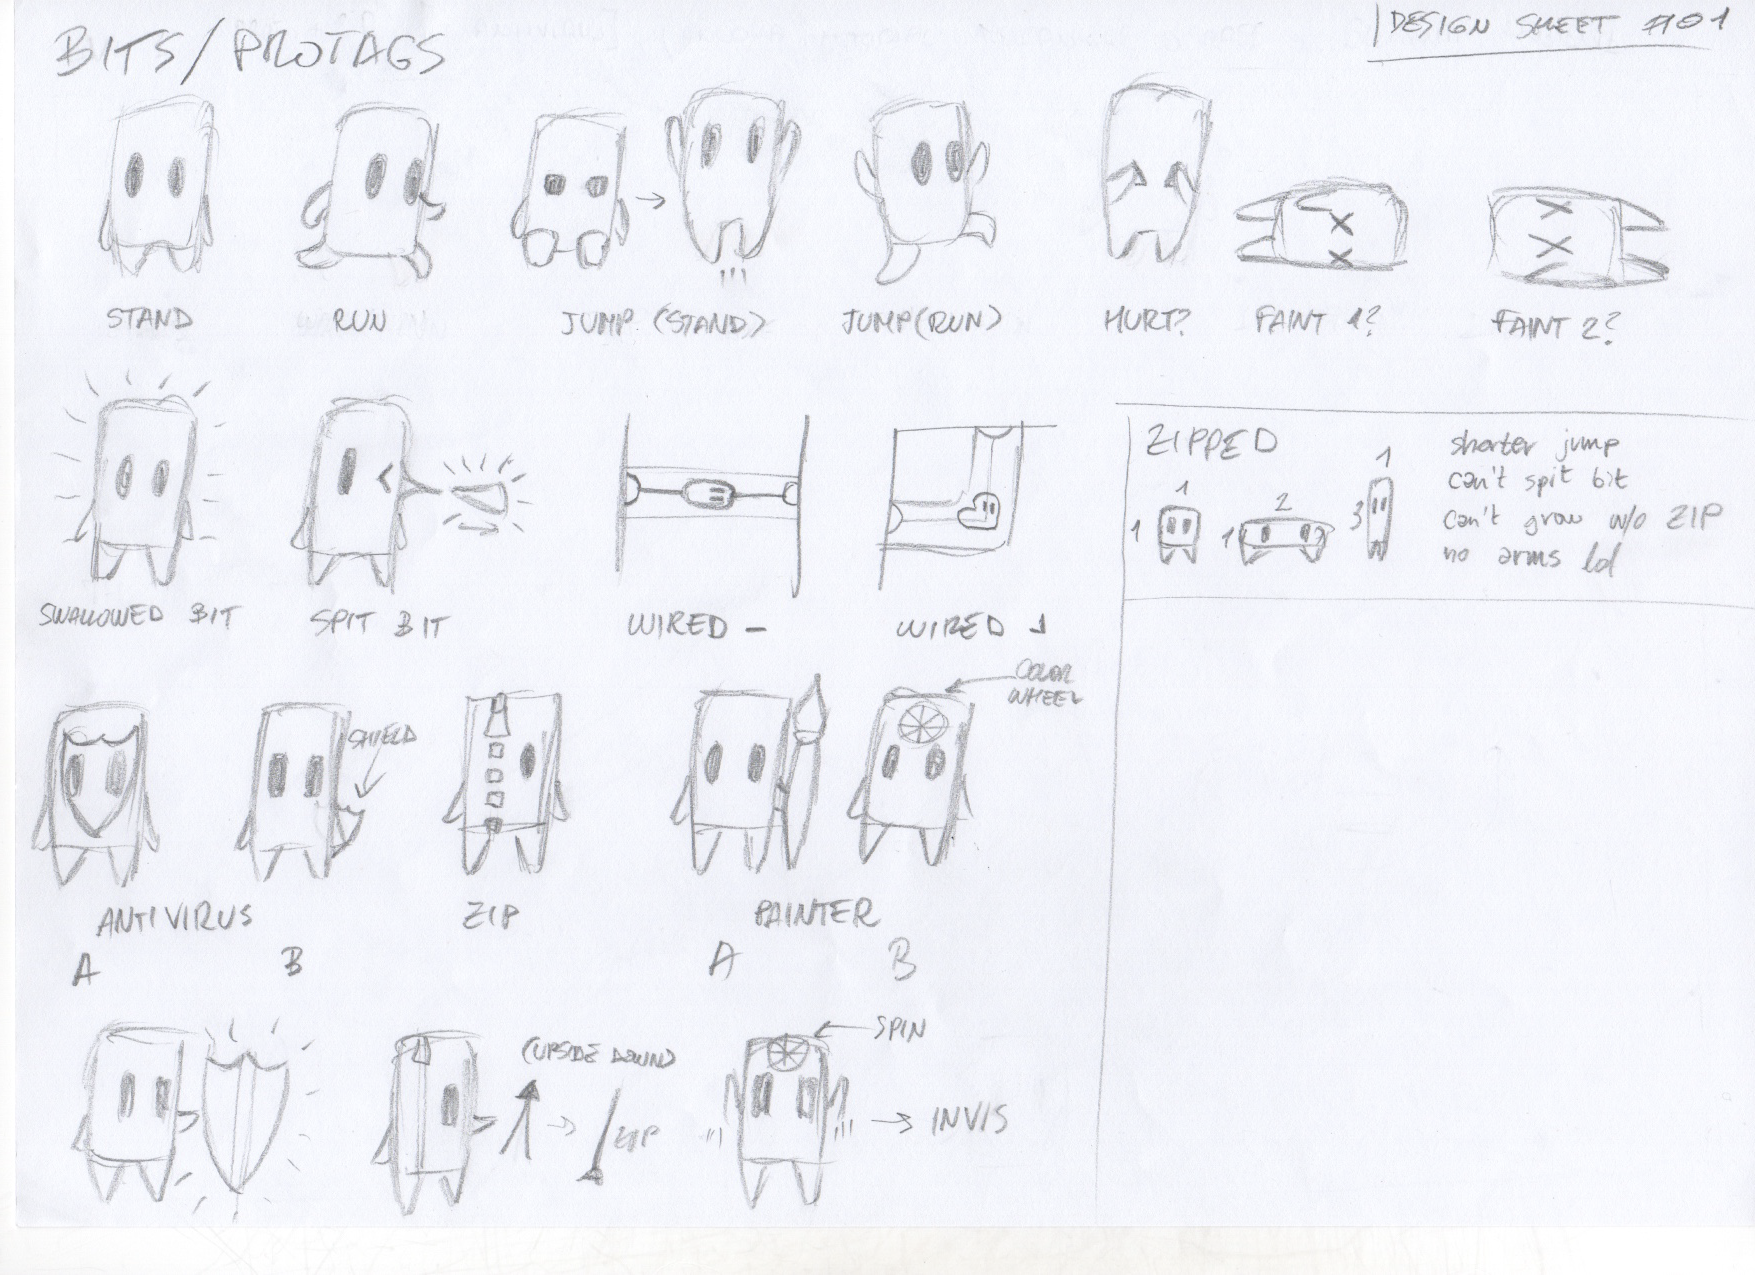
\includegraphics[width=0.5\textwidth]{images/Characters}
\end{figure}
	\begin{figure}[H]
	\centering
	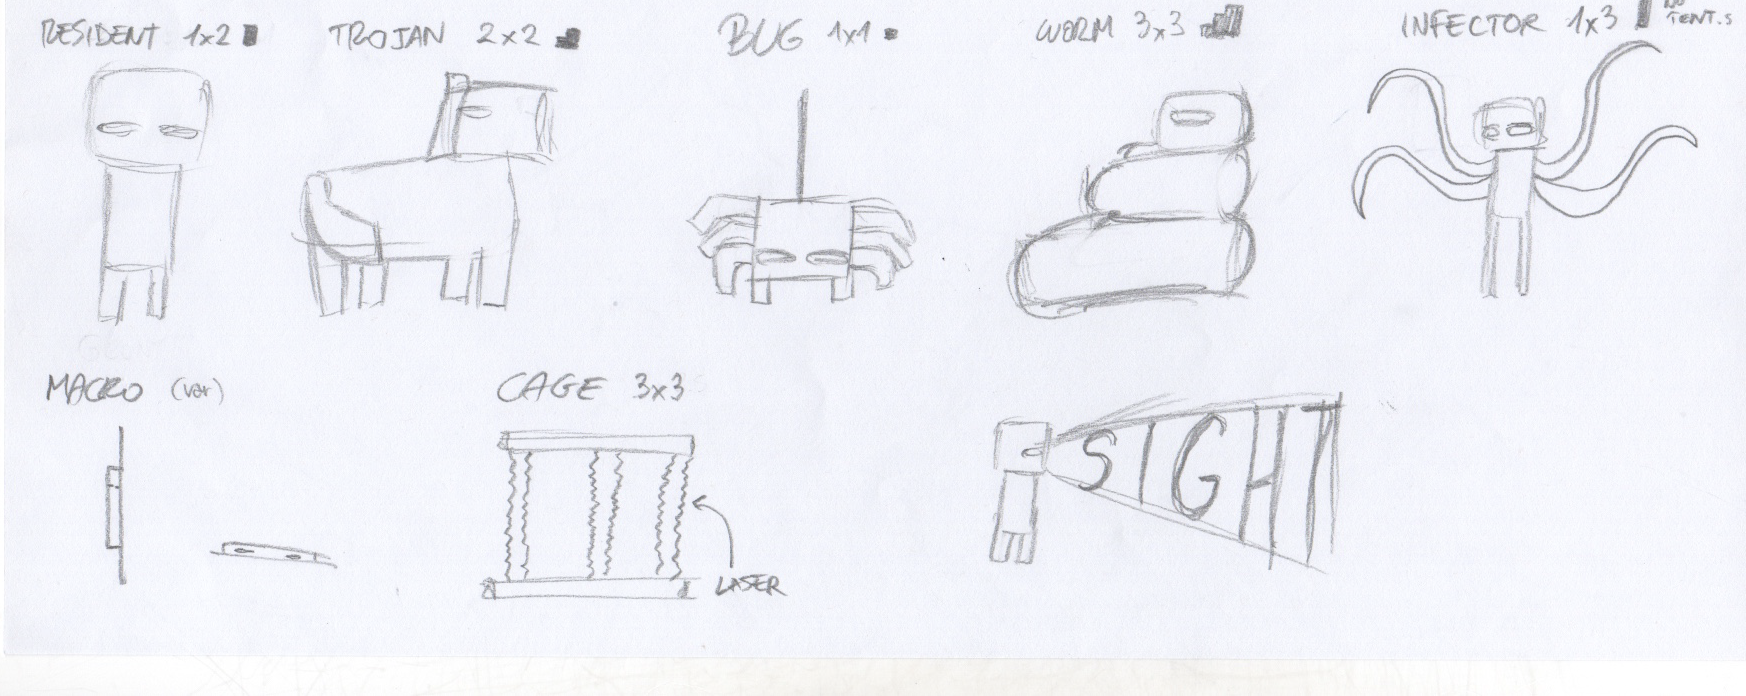
\includegraphics[width=0.5\textwidth]{images/Enemy}
\end{figure}
	\begin{figure}[H]
	\centering
	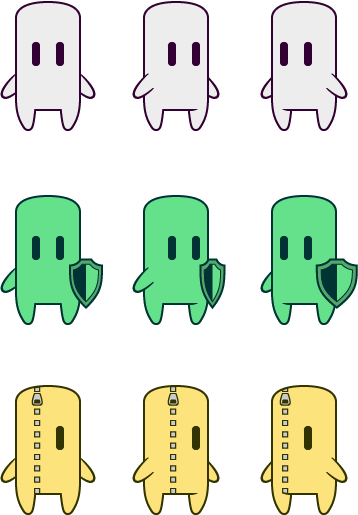
\includegraphics[width=0.3\textwidth]{images/Bits}
\end{figure}


\chapter{Sound Overview}
The background music is taken from the electro genre, avoiding too much powerful tracks but looking for some more relaxing ones. This genre should be perfect to make the player feeling to be in a virtual world and to improve his focus on solving the puzzles. The sound effects are similar to platformers like Super Mario and to arcade games.


\end{document}
